% =====================================================================
\chapter{Funciones de varias variables, límites y continuidad}
\label{tema:3}
% =====================================================================

Una función de varias variables asigna un número a cada punto del plano o del espacio: la altitud de un terreno, la temperatura de una habitación o la pérdida de una red neuronal en función de sus parámetros. Este tema enseña a visualizarlas mediante gráficas y curvas de nivel y extiende a ellas las nociones de límite y continuidad. La novedad respecto a una variable es que un punto puede alcanzarse por infinitos caminos, y el límite debe ser el mismo por todos ellos. La presentación sigue las §4.1--4.2 de OpenStax~\cite{openstax3}, las sesiones~24--25 de 18.02SC~\cite{mit1802}, el capítulo~8 de Apostol~\cite{apostol2} y la §13.1 de Strang~\cite{strangcalc}.

\section{Funciones, dominio y gráfica}

\begin{definicion}[Función de varias variables]\label{def:funcion-n}
Una \emph{función real de $n$ variables} es una regla $f$ que asigna a cada punto $\vx=(x_1,\dots,x_n)$ de un conjunto $D\subseteq\R^n$, su \emph{dominio}, un único número real $f(\vx)$. Si no se indica, el dominio es el mayor conjunto en el que la fórmula tiene sentido. La \emph{imagen} es $\{f(\vx):\vx\in D\}$. Para $n=2$, la \emph{gráfica} de $f$ es la superficie $\{(x,y,z)\in\R^3: (x,y)\in D,\ z=f(x,y)\}$.
\end{definicion}

\begin{ejemplo}\label{ej:t3-graficas}
(a) $f(x,y)=x^2+y^2$ tiene dominio $\R^2$, imagen $[0,\infty)$ y gráfica un \emph{paraboloide} de vértice el origen. (b) $g(x,y)=\sqrt{1-x^2-y^2}$ exige $x^2+y^2\le1$: su dominio es el disco unidad cerrado, su imagen $[0,1]$ y su gráfica la semiesfera superior de radio~1, pues $z=g(x,y)$ equivale a $x^2+y^2+z^2=1$ con $z\ge0$. (c) $h(x,y)=ax+by+c$ es una función \emph{afín}; su gráfica es el plano $z=ax+by+c$.
\end{ejemplo}

\section{Curvas y superficies de nivel}

\begin{definicion}[Conjuntos de nivel]\label{def:nivel}
Sea $f:D\subseteq\R^n\to\R$ y $c\in\R$. El \emph{conjunto de nivel} $c$ de $f$ es $\{\vx\in D: f(\vx)=c\}$. Para $n=2$ se llama \emph{curva de nivel}, y para $n=3$, \emph{superficie de nivel}. Un \emph{mapa de contorno} dibuja varias curvas de nivel, normalmente para valores de $c$ igualmente espaciados.
\end{definicion}

La curva de nivel $c$ es la proyección sobre el plano $xy$ del corte de la gráfica con el plano horizontal $z=c$, como las curvas de un mapa topográfico. Dos curvas de nivel distintas nunca se cortan, porque $f$ asigna un único valor a cada punto. Donde las curvas de nivel (equiespaciadas) están más juntas, la función cambia más deprisa.

\begin{figure}[ht]
\centering
\begin{tikzpicture}[scale=0.85,font=\small]
  \begin{scope}
    \draw[->] (-2.3,0) -- (2.3,0) node[right] {$x$};
    \draw[->] (0,-2.3) -- (0,2.3) node[above] {$y$};
    \foreach \c in {1,2,3,4} \draw[thick] (0,0) circle ({0.5*sqrt(\c)*2});
    \node at (0,-2.75) {$x^2+y^2=c$, \ $c=1,2,3,4$};
  \end{scope}
  \begin{scope}[xshift=6.5cm]
    \draw[->] (-2.3,0) -- (2.3,0) node[right] {$x$};
    \draw[->] (0,-2.3) -- (0,2.3) node[above] {$y$};
    \foreach \c in {0.5,1.5} {
      \draw[thick,domain=-1.2:1.2,smooth,variable=\t] plot ({sqrt(\c)*cosh(\t)},{sqrt(\c)*sinh(\t)});
      \draw[thick,domain=-1.2:1.2,smooth,variable=\t] plot ({-sqrt(\c)*cosh(\t)},{sqrt(\c)*sinh(\t)});
      \draw[thick,dashed,domain=-1.2:1.2,smooth,variable=\t] plot ({sqrt(\c)*sinh(\t)},{sqrt(\c)*cosh(\t)});
      \draw[thick,dashed,domain=-1.2:1.2,smooth,variable=\t] plot ({sqrt(\c)*sinh(\t)},{-sqrt(\c)*cosh(\t)});
    }
    \draw[gray] (-2,-2) -- (2,2); \draw[gray] (-2,2) -- (2,-2);
    \node at (0,-2.75) {$x^2-y^2=c$, \ $c=\pm\tfrac12,\pm\tfrac32$ y $0$};
  \end{scope}
\end{tikzpicture}
\caption{Curvas de nivel del paraboloide $x^2+y^2$ (circunferencias, cada vez más juntas porque la función crece cada vez más deprisa) y de la silla $x^2-y^2$ (hipérbolas: trazo continuo para $c>0$, discontinuo para $c<0$; el nivel~$0$ son las dos diagonales).}
\label{fig:t3-niveles}
\end{figure}

\begin{ejemplo}\label{ej:t3-niveles}
Para $f(x,y)=x^2+y^2$, la curva de nivel $c$ es vacía si $c<0$, el origen si $c=0$ y la circunferencia de radio $\sqrt c$ si $c>0$. Para $f(x,y)=x^2-y^2$, los niveles $c\neq0$ son hipérbolas y el nivel~0 es el par de rectas $y=\pm x$ (\cref{fig:t3-niveles}). Para $F(x,y,z)=x^2+y^2+z^2$, las superficies de nivel $c>0$ son esferas de radio $\sqrt c$.
\end{ejemplo}

\section{Límites}

En $\R^n$ la cercanía se mide con la norma euclídea: la \emph{bola abierta} de centro $\va$ y radio $\delta>0$ es $B(\va,\delta)=\{\vx:\norm{\vx-\va}<\delta\}$. Se dice que $\va$ es un \emph{punto de acumulación} de $D$ si toda bola centrada en $\va$ contiene puntos de $D$ distintos de $\va$.

\begin{definicion}[Límite]\label{def:limite-n}
Sea $f:D\subseteq\R^n\to\R$ y $\va$ un punto de acumulación de $D$. Se dice que $\lim_{\vx\to\va}f(\vx)=L$ si para cada $\varepsilon>0$ existe $\delta>0$ tal que
\[
\vx\in D,\quad 0<\norm{\vx-\va}<\delta\ \Longrightarrow\ \abs{f(\vx)-L}<\varepsilon .
\]
\end{definicion}

La definición es la de una variable con $\abs{x-a}$ sustituido por $\norm{\vx-\va}$, y las demostraciones de las reglas algebraicas (límite de la suma, del producto, del cociente con denominador de límite no nulo) se trasladan sin cambios. Dos hechos elementales se usan constantemente: para $\vx=(x,y)$ y $\va=(a,b)$,
\begin{equation}\label{eq:t3-coordenada}
\abs{x-a}\le\norm{\vx-\va},\qquad \abs{y-b}\le\norm{\vx-\va},
\end{equation}
porque $\norm{\vx-\va}^2=(x-a)^2+(y-b)^2$ es mayor o igual que cada sumando.

\begin{proposicion}[Acotación]\label{prop:acotacion}
Si $\abs{f(\vx)-L}\le g(\vx)$ para $\vx$ cerca de $\va$ y $\lim_{\vx\to\va}g(\vx)=0$, entonces $\lim_{\vx\to\va}f(\vx)=L$.
\end{proposicion}

\begin{proof}
Dado $\varepsilon>0$, sea $\delta>0$ tal que $0<\norm{\vx-\va}<\delta$ implica $g(\vx)<\varepsilon$ (achicando $\delta$ si hace falta para que valga también la cota del enunciado). Para esos $\vx$, $\abs{f(\vx)-L}\le g(\vx)<\varepsilon$.
\end{proof}

En el origen es útil pasar a \emph{coordenadas polares} $x=r\cos\theta$, $y=r\sin\theta$, con $r=\norm{(x,y)}$: si $\abs{f(r\cos\theta,r\sin\theta)-L}\le h(r)$ con $h(r)\to0$ cuando $r\to0^+$ y la cota $h$ \emph{no depende de $\theta$}, el límite es $L$ por la \cref{prop:acotacion}.

\begin{ejemplo}\label{ej:t3-polares}
$\lim_{(x,y)\to(0,0)}\dfrac{x^2y}{x^2+y^2}=0$. En polares, $\dfrac{x^2y}{x^2+y^2}=\dfrac{r^3\cos^2\theta\sin\theta}{r^2}=r\cos^2\theta\sin\theta$, cuyo valor absoluto es menor o igual que $r$, y $r\to0$.
\end{ejemplo}

\begin{teorema}[Límites a lo largo de curvas]\label{teo:trayectorias}
Sea $\lim_{\vx\to\va}f(\vx)=L$ y sea $\boldsymbol\gamma:(0,\eta)\to D$ una curva con $\boldsymbol\gamma(t)\neq\va$ y $\lim_{t\to0^+}\boldsymbol\gamma(t)=\va$. Entonces $\lim_{t\to0^+}f(\boldsymbol\gamma(t))=L$.
\end{teorema}

\begin{proof}
Dado $\varepsilon>0$, sea $\delta$ el de la \cref{def:limite-n}. Como $\boldsymbol\gamma(t)\to\va$, existe $t_0>0$ tal que $0<t<t_0$ implica $\norm{\boldsymbol\gamma(t)-\va}<\delta$; además $\boldsymbol\gamma(t)\neq\va$, luego $0<\norm{\boldsymbol\gamma(t)-\va}<\delta$ y $\abs{f(\boldsymbol\gamma(t))-L}<\varepsilon$.
\end{proof}

\begin{corolario}[Criterio de no existencia]\label{cor:no-existe}
Si a lo largo de dos curvas que llegan a $\va$ la función tiene límites distintos (o a lo largo de una no tiene límite), entonces $\lim_{\vx\to\va}f(\vx)$ no existe.
\end{corolario}

\begin{ejemplo}\label{ej:t3-no-existe}
(a) Sea $f(x,y)=\dfrac{xy}{x^2+y^2}$. Sobre la recta $y=mx$ ($x\neq0$), $f(x,mx)=\dfrac{mx^2}{(1+m^2)x^2}=\dfrac{m}{1+m^2}$, que depende de $m$: vale $0$ sobre el eje $x$ y $\tfrac12$ sobre la diagonal. El límite en el origen no existe.

(b) Sea $g(x,y)=\dfrac{x^2y}{x^4+y^2}$. Sobre cualquier recta $y=mx$, $g(x,mx)=\dfrac{mx}{x^2+m^2}\to0$ (y sobre el eje $y$, $g=0$). Sin embargo, sobre la parábola $y=x^2$, $g(x,x^2)=\dfrac{x^4}{2x^4}=\tfrac12$. El límite no existe, aunque por todas las rectas valga~0.
\end{ejemplo}

\section{Continuidad}

\begin{definicion}[Continuidad]\label{def:continua-n}
Una función $f:D\to\R$ es \emph{continua en} $\va\in D$ si $\lim_{\vx\to\va}f(\vx)=f(\va)$ (o si $\va$ es un punto aislado de $D$). Es continua en $D$ si lo es en cada punto de $D$.
\end{definicion}

\begin{proposicion}[Funciones continuas elementales]\label{prop:continuas}
\begin{enumerate}
  \item Las proyecciones $(x,y)\mapsto x$ y $(x,y)\mapsto y$ son continuas en $\R^2$.
  \item Sumas, productos y cocientes (donde el denominador no se anula) de funciones continuas son continuos. En particular, los polinomios en $x$ e $y$ son continuos en $\R^2$, y las funciones racionales lo son en su dominio.
  \item Si $g$ es continua en $\va$ y $h:\R\to\R$ es continua en $g(\va)$, entonces $h\circ g$ es continua en $\va$.
\end{enumerate}
\end{proposicion}

\begin{proof}[Idea de la demostración]
(i) Por~\eqref{eq:t3-coordenada}, basta tomar $\delta=\varepsilon$. (ii) Son las reglas algebraicas de los límites. (iii) Es el argumento de una variable con normas (\cref{eje:3-composicion}).
\end{proof}

Así, $e^{x^2+y^2}$, $\sin(xy)$ o $\ln(1+x^2+y^2)$ son continuas en todo $\R^2$, y para calcular su límite en un punto basta sustituir. Los casos interesantes son los cocientes en puntos donde se anula el denominador, como en los ejemplos anteriores.

\begin{ejemplo}\label{ej:t3-trozos}
La función $f(x,y)=\dfrac{x^2y}{x^2+y^2}$ si $(x,y)\neq(0,0)$, $f(0,0)=0$, es continua en $\R^2$: fuera del origen es racional con denominador no nulo, y en el origen su límite es $0=f(0,0)$ (\cref{ej:t3-polares}). En cambio, $\dfrac{xy}{x^2+y^2}$ no puede extenderse de forma continua al origen, cualquiera que sea el valor que se le asigne (\cref{ej:t3-no-existe}).
\end{ejemplo}

\begin{observacion}[Errores frecuentes]
\begin{enumerate}[label=(\alph*)]
\item Comprobar que el límite vale lo mismo por todas las rectas \emph{no} demuestra que exista (\cref{ej:t3-no-existe}(b)). Las trayectorias solo sirven para refutar; para demostrar hay que acotar.
\item En polares, la cota debe ser independiente de $\theta$. Por ejemplo, $\dfrac{xy}{x^2+y^2}=\cos\theta\sin\theta$ no depende de $r$, pero sí de $\theta$: no tiene límite.
\item Los límites iterados $\lim_x\lim_y f$ y $\lim_y\lim_x f$ pueden existir y coincidir sin que exista el límite doble.
\end{enumerate}
\end{observacion}

\begin{observacion}[Conexión con el curso]
La pérdida de un modelo es una función de todos sus parámetros, y su mapa de curvas de nivel describe la geometría que recorre el entrenamiento: valles alargados (curvas de nivel elípticas muy excéntricas) explican la lentitud del descenso de gradiente y motivan los métodos de los módulos~4 y~7. Una función que se usa constantemente en el curso es la \emph{log-suma-exp} $\ln(e^{x}+e^{y})$, versión suave del máximo (\cref{eje:3-lse}), cuyo gradiente es la función softmax (módulo~1, tema~4; módulo~4).
\end{observacion}

\begin{lecturas}
\item OpenStax \emph{Calculus}, vol.~3~\cite{openstax3}, §4.1 «Functions of Several Variables» y §4.2 «Limits and Continuity».
\item MIT 18.02SC~\cite{mit1802}, unidad~2, parte~A, sesiones~24 y~25 (gráficas, curvas de nivel y mapas de contorno).
\item Apostol~\cite{apostol2}, cap.~8, para la definición de límite con bolas abiertas y la continuidad de funciones de varias variables.
\item Strang, \emph{Calculus}~\cite{strangcalc}, §13.1 «Surface and Level Curves».
\end{lecturas}

\section*{Ejercicios del tema 3}
\addcontentsline{toc}{section}{Ejercicios del tema 3}

\begin{ejercicio}{1}{eje:3-conceptos}
Razone si son verdaderas o falsas: (a) dos curvas de nivel distintas de una misma función pueden cortarse; (b) si el límite de $f$ en el origen vale~$0$ a lo largo de todas las rectas que pasan por él, entonces $\lim_{(x,y)\to(0,0)}f(x,y)=0$; (c) la gráfica de una función $f:\R^2\to\R$ es un subconjunto de $\R^3$, y sus curvas de nivel, subconjuntos de $\R^2$.
\end{ejercicio}

\begin{ejercicio}{2}{eje:3-dominios}
Determine y dibuje el dominio, e indique la imagen, de: (a) $\sqrt{1-x^2-y^2}$; (b) $\ln(x-y)$; (c) $\dfrac{1}{xy}$; (d) $\sqrt{y-x^2}$.
\end{ejercicio}

\begin{ejercicio}{2}{eje:3-niveles}
Dibuje las curvas de nivel indicadas y describa la gráfica: (a) $1-x-y$, niveles $c=-1,0,1$; (b) $x^2+y^2$, niveles $c=0,1,4$; (c) $1-x^2-y^2$, niveles $c=1,0,-3$; (d) $x^2-y^2$, niveles $c=-1,0,1$.
\fuente{adaptado de MIT 18.02SC~\cite{mit1802}, problemas suplementarios, 2A-1.}
\end{ejercicio}

\begin{ejercicio}{2}{eje:3-niveles-2}
Describa los conjuntos de nivel de: (a) $f(x,y)=x^2+4y^2$; (b) $g(x,y)=y-x^2$; (c) $h(x,y)=2x+y$ (¿qué relación hay entre la normal a estas rectas y los coeficientes?); (d) $F(x,y,z)=x^2+y^2+z^2$.
\fuente{adaptado de OpenStax \emph{Calculus}, vol.~3~\cite{openstax3}, §4.1.}
\end{ejercicio}

\begin{ejercicio}{2}{eje:3-onda}
Sea $F(x,t)=\cos^2(x-ct)$ con $c>0$, donde $x$ es la posición sobre una cuerda y $t$ el tiempo. (a) Describa las curvas de nivel de $F$ en el plano $(x,t)$. (b) Compare las gráficas de $x\mapsto F(x,t)$ para $t=-1,0,1$ cuando $c=2$ y explique qué fenómeno describe $F$.
\fuente{adaptado de MIT 18.02SC~\cite{mit1802}, \emph{problem set}~4, parte~II, problema~1.}
\end{ejercicio}

\begin{ejercicio}{2}{eje:3-interseccion-superficies}
Las superficies $z=x^2-y^2$ y $z=2+(x-y)^2$ se cortan en una curva. (a) Demuestre que la proyección de la curva sobre el plano $xy$ está contenida en $y(x-y)=1$. (b) Parametrice la curva tomando $y=t$ y compruebe que pasa por $(2,1,3)$.
\fuente{adaptado de MIT 18.02SC~\cite{mit1802}, \emph{problem set}~4, parte~II, problema~2.}
\end{ejercicio}

\begin{ejercicio}{2}{eje:3-limites-directos}
Calcule, justificando la continuidad o simplificando previamente: (a) $\lim_{(x,y)\to(1,2)}\dfrac{x^2y+3}{1+xy}$; (b) $\lim_{(x,y)\to(0,0)}e^{x+y}\cos(xy)$; (c) $\lim_{(x,y)\to(1,1)}\dfrac{x^2-y^2}{x-y}$, con $x\neq y$; (d) $\lim_{(x,y)\to(4,4)}\dfrac{x-y}{\sqrt x-\sqrt y}$, con $x\neq y$.
\fuente{adaptado de OpenStax \emph{Calculus}, vol.~3~\cite{openstax3}, §4.2.}
\end{ejercicio}

\begin{ejercicio}{2}{eje:3-no-existe}
Demuestre que no existen los límites en el origen de: (a) $\dfrac{x^2-y^2}{x^2+y^2}$; (b) $\dfrac{xy^2}{x^2+y^4}$. (Indicación: en (b), pruebe las curvas $x=my^2$.)
\fuente{adaptado de OpenStax \emph{Calculus}, vol.~3~\cite{openstax3}, §4.2.}
\end{ejercicio}

\begin{ejercicio}{2}{eje:3-polares}
Calcule los límites en el origen, pasando a polares: (a) $\dfrac{x^3}{x^2+y^2}$; (b) $\dfrac{x^2y^2}{x^2+y^2}$; (c) $\dfrac{xy}{\sqrt{x^2+y^2}}$; (d) $(x^2+y^2)\ln(x^2+y^2)$.
\end{ejercicio}

\begin{ejercicio}{2}{eje:3-continuidad}
(a) Sea $f(x,y)=\dfrac{x^3+y^3}{x^2+y^2}$ fuera del origen y $f(0,0)=a$. ¿Para qué valor de $a$ es $f$ continua en $\R^2$? (b) ¿Existe algún valor $b$ que haga continua en el origen la función $g(x,y)=\dfrac{x^2-y^2}{x^2+y^2}$, $g(0,0)=b$?
\end{ejercicio}

\begin{ejercicio}{2}{eje:3-lse}
Sea $f(x,y)=\ln(e^x+e^y)$. (a) Demuestre que $\max(x,y)\le f(x,y)\le\max(x,y)+\ln2$. (b) Describa la curva de nivel $f=0$ como gráfica $y=\varphi(x)$, indicando su dominio y sus asíntotas. (c) Calcule $f(10,0)$ y $f(1,1)$ y compare con $\max(x,y)$.
\end{ejercicio}

\begin{ejercicio}{3}{eje:3-epsilon-delta}
Demuestre con la \cref{def:limite-n} (dando $\delta$ en función de $\varepsilon$) que: (a) $\lim_{(x,y)\to(1,1)}(2x+3y)=5$; (b) $\lim_{(x,y)\to(0,0)}\dfrac{x^2y}{x^2+y^2}=0$.
\end{ejercicio}

\begin{ejercicio}{3}{eje:3-composicion}
(a) Demuestre la \cref{prop:continuas}(iii): si $g:\R^2\to\R$ es continua en $\va$ y $h:\R\to\R$ es continua en $g(\va)$, entonces $h\circ g$ es continua en $\va$. (b) Deduzca que $e^{-(x^2+y^2)}$ es continua en $\R^2$, suponiendo conocida la continuidad de los polinomios.
\end{ejercicio}

\begin{ejercicio}{3}{eje:3-cuadratica}
Sea $f(x,y)=x^2+xy+y^2$. (a) Demuestre que $\tfrac12(x^2+y^2)\le f(x,y)\le\tfrac32(x^2+y^2)$ para todo $(x,y)$. (Indicación: $\abs{xy}\le\frac12(x^2+y^2)$.) (b) Deduzca que cada curva de nivel $f=c>0$ está contenida en la corona $\frac{2c}{3}\le x^2+y^2\le 2c$, y que $f(x,y)>0$ salvo en el origen.
\end{ejercicio}

\begin{ejercicio}{3}{eje:3-trayectorias}
Sea $f(x,y)=\dfrac{x^4y^4}{(x^2+y^4)^3}$ fuera del origen. (a) Demuestre que $f\to0$ a lo largo de toda recta que pasa por el origen. (b) Calcule el límite de $f$ a lo largo de la curva $x=y^2$ y concluya, con el \cref{cor:no-existe}, que el límite en el origen no existe.
\end{ejercicio}
